\chapter{Introdução}

Com o passar dos anos, principalmente em uma época onde a tecnologia e os negócios mudam e evoluem de modo extremamente rápido, o mercado demanda e espera software inovadores e de alta qualidade, que sejam adequados a suas necessidades $-$ e o mais rápido possível \cite{TheBusinessOfInnovation}.

O desenvolvimento ágil de software, que neste ano de 2012 completa 11 anos, foi elaborado \cite{AgileManifesto} visando atender à estas expectativas do mercado, focando o processo de desenvolvimento nas pessoas e abraçando as mudanças que  naturalmente surgem durante a construção do software. De acordo com \citeonline{PMNetworkFailureDrop}, o \textit{Chaos Manifesto 2011}\footnote{O \textit{Chaos Manifesto} é uma pesquisa bienal realizada pelo \textit{The Standish Group} e teve início em 1994. As pesquisas publicadas em um ano representam os dados do ano anterior.} mostra que os resultados de 2010 representam, desde sua primeira edição, a maior taxa de sucesso nos projetos de desenvolvimento de software, que aumentou de 32\% em 2008 para 37\% em 2010. Segundo \citeonline{ResumoChaosReport}, o \textit{The Standish Group} conclui que uma das razões para o aumento da taxa de sucesso foi a utilização das metodologias ágeis, que cresce a uma taxa de 22\% CAGR\footnote{\href{http://en.wikipedia.org/wiki/Compound_annual_growth_rate} {Compound annual growth rate}} e hoje são adotados em 9\% de todos os projetos de Tecnologia da Informação em andamento e em 29\% dos novos projetos.

Como a adoção do desenvolvimento ágil é crescente nos últimos anos, diversos métodos e técnicas vem sendo desenvolvidos tendo como base os princípios e valores ágeis \cite{BDDRodrigo}, principalmente relacionadas ao teste de software. Este trabalho pretende contribuir e contextualizar a utilização de técnicas emergentes de teste de software, aqui definidas como Desenvolvimento Guiado por Testes (do inglês, \textit{Test-Driven Development} - TDD)\nomenclature{TDD}{Test-Driven Development}, Desenvolvimento Guiado por Comportamento (do inglês, \textit{Behaviour-Driven Development - BDD})\nomenclature{BDD}{Behaviour-Driven Development}, Integração Contínua e Dublês de Teste. Para esta contextualização, sera utilizada um sistema web desenvolvido utilizando tais técnicas: O kanban-roots.

\section{Justificativas e objetivos}

Na literatura são encontrados alguns poucos trabalhos relacionados ao tema que estamos querendo abordar nesta monografia, como constata \citeonline{BDDSolis}. Sendo assim, o objetivo do presente trabalho é oferecer um estudo teórico prático das novas tendências/técnicas emergentes na área de teste de software com metodologias ágeis de desenvolvimento. Em vistas de agregar conhecimentos, ora dispersos e difusos, sobre as diferentes abordagens, possibilidades e pontos em aberto no emprego de tais técnicas.

As técnicas que serão abordadas neste trabalho tem seu conceito definido no mercado e evoluem através da evolução das ferramentas que os implementam. O fluxo de evolução é o seguinte:

\begin{figure}[h]
  \center
  \caption{Fluxo de evolução dos conceitos e ferramentas}
  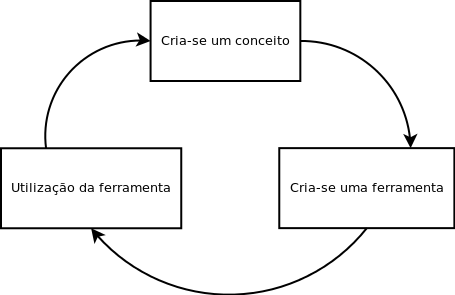
\includegraphics[scale=0.60]{images/fluxo-conceito-ferramenta}
  \label{img:fluxo_conceito_ferramenta}
\end{figure}

Primeiramente cria-se um conceito e, em seguida, uma ferramenta que o implemente. Com base na utilização e observação desta ferramenta, há uma percepção de novas necessidades, fazendo que os conceitos evoluam e novas ferramentas sejam criadas.

Desta forma, a evolução das ferramentas e a evolução conceitual estão intimamente ligadas. No texto original sobre BDD \cite{IntroducingBDD} já se encontra isto. A inspiração para a criação de BDD foi uma ferramenta chamada \textit{AgileDox}\footnote{Mais informações em \url{http://agiledox.sourceforge.net}}, que fez o autor antever as novas possibilidades que cristalizou no conceito de BDD. Justamente por esta característica dinâmica, a informação e os diferentes conceitos estão dispersos, pois nunca foram sistematizados, ficando em uma espécie de ``inteligência coletiva"\ da comunidade de desenvolvimento ágil.

Além disso, como o presente trabalho está no contexto dos métodos ágeis, e nestes as partes conceitual e prática formam um todo inseparável, para toda técnica abordada serão exemplificados os conceitos usando o código de uma ferramenta web desenvolvida pelo próprio autor, utilizando práticas ágeis de desenvolvimento, especificamente Desenvolvimento guiado por Testes (TDD) e Desenvolvimento guiado por Comportamento (BDD); denominada kanban-roots.

\section{Metodologia}

Para atingirmos os objetivos propostos neste trabalho, será feita uma explanação sobre cada uma das técnicas emergentes estudadas, aqui definidas como:

\begin{itemize}
  \item Desenvolvimento guiado por testes (TDD, do inglês \textit{Test-Driven Development})
  \item Desenvolvimento guiado por comportamento (BDD, do inglês \textit{Behaviour-Driven Development}
  \item Integração contínua
  \item Dublês de teste
\end{itemize}

Serão comparadas as diferentes abordagens, possibilidades, pontos em aberto no emprego de cada técnica assim como observando a aplicabilidade de cada uma delas e a eficiência respectiva.

Como base para a discussão, será utilizado o kanban-roots\footnote{\url{http://github.com/hugomaiavieira/kanban-roots}}, que será apresentado na Seção \ref{sec:kanban_roots}. O kanban-roots é um projeto que foi desenvolvido pelo autor do presente trabalho utilizando todas as técnicas abordadas neste, possibilitando desta forma a obtenção de dados e experiências da utilização das técnicas em um projeto real.

Todos os trechos de código apresentados neste trabalho são trechos retirados do kanban-roots e a primeira linha de cada trecho sempre será um comentário informando o nome do arquivo original em que o dado trecho se encontra.

\section{Ferramentas utilizadas}

Para o desenvolvimento do kanban-roots foram utilizadas diversas ferramentas, sendo importante citar em que contexto e momento cada uma delas é utilizada.

Como base para o desenvolvimento, foi utilizado o \textit{framework web} Ruby On Rails\footnote{\url{http://rubyonrails.org}}. Para os testes de unidade apresentados na Seção \ref{sub:tdd} foi utilizado o Test::Unit\footnote{\url{http://test-unit.rubyforge.org/}}. Já na Seção \ref{sub:bdd} é utilizado o Rspec\footnote{\url{http://rspec.info/}} para testes unitários, testes de aceitação e dublês de teste. Ainda na Seção \ref{sub:bdd} também foi utilizado o Cucumber\footnote{\url{http://cukes.info/}} para testes de aceitação. Além dessas ferramentas, também foi utilizado o FactoryGirl\footnote{\url{https://github.com/thoughtbot/factory_girl}} para \textit{fixtures replacement} em todos os momentos em que se fez necessário.

\section{Organização}
\label{sec:organizacao}

\textbf{TODO: Falar como a monografia está organizada: no capítulo tal, será abordado isso, isso e aquilo. Na seção tal bla bla bla.}